\documentclass[tikz]{standalone}
\usetikzlibrary{automata,positioning}
\begin{document}

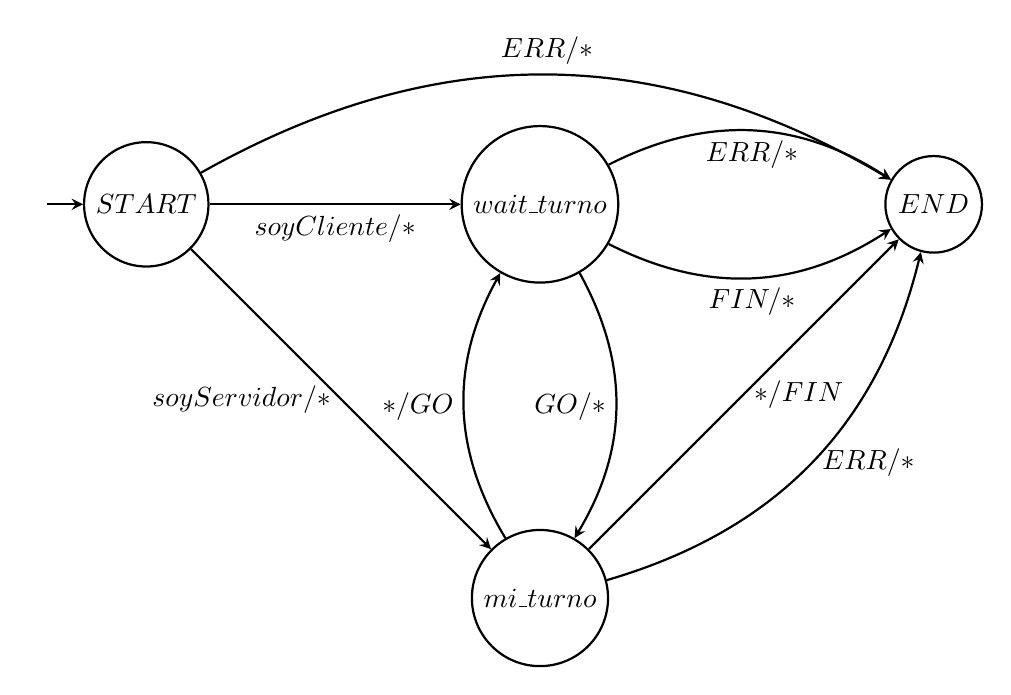
\begin{tikzpicture}[>=stealth,node distance=8cm,on grid,auto, thick, initial text=] 
  \node[state,initial] (q_0)   {$START$}; 
  \node[state]         (q_1) [right=5cm of q_0] {$wait\_turno$};
  \node[state]         (q_2) [below=5cm of q_1] {$mi\_turno$};
  \node[state]         (q_3) [right=5cm of q_1] {$END$};

  \path[->]            (q_0) edge [bend left] node[above] {$ERR/*$} (q_3)
  					   (q_1) edge [bend left] node[below] {$ERR/*$} (q_3)
  					   (q_1) edge [bend right] node[below] {$FIN/*$} (q_3)
  					   (q_0) edge [left] node[below] {$soyCliente/*$} (q_1)
  					   (q_0) edge [left] node[left] {$soyServidor/*$} (q_2)
  					   (q_1) edge [bend left] node[left] {$GO/*$} (q_2)
  					   (q_2) edge [bend left] node[left] {$*/GO$} (q_1)
  					   (q_2) edge [bend right] node[right] {$ERR/*$} (q_3)
  					   (q_2) edge [right] node [right] {$*/FIN$} (q_3);
\end{tikzpicture}
\end{document}